\section{WERYFIKACJA PRACY PROGRAMU}
\label{testSection}

\subsection{Testy jednostkowe}

Działanie wszystkich funkcji wchodzących w skład bardziej skomplikowanej logiki
biznesowej programu, zawartej w module \verb|algorithms| zostało zweryfikowane
testami jednostkowymi. Wynik wykonania testów jednostkowych można zobaczyć na
listingu \ref{cargoTestListing}.

\lstinputlisting[
    float=h!,
    basicstyle=\ttfamily\small,
    frame=tb,
    label={cargoTestListing},
    caption={Wykonanie testów jednostkowych}
]{./code/cargoTest.txt}

Działanie testów jednostkowych można opisać następująco:

\begin{itemize}

    \item \verb|mermaid_diagram_generation::tests::works| - test sprawdza
        poprawność działania algorytmu generującego diagram ER w składni
        \verb|mermaid.js|. Do implementacji podawana jest przykładowa struktura
        tabel. Sprawdzane jest, czy wygenerowany diagram jest poprawny.

    \item \verb|sql_variable_parser::tests::parsing_test| - test sprawdza
        podstawową funkcję parsującą SQL wykorzystywaną do implementacji
        bardziej skomplikowanej funkcjonalności parsera.

    \item \verb|sql_variable_parser::tests::parsing_multiple| - test sprawdza
        poprawne działanie parsera SQL, gdy w jednym zapytaniu znajduje się
        większa ilość odwołań do zmiennych.

    \item \verb|sql_variable_parser::tests::bind_vec| - test sprawdza poprawność
        działania funkcji, która przekształca tablicę mieszającą zawierającą
        dostępne zmienne i sparsowany SQL na tablicę wartości, które powinny
        zostać wysłane do bazy danych.

    \item \verb|sql_variable_parser::tests::parsing_endpoint_info| - test
        sprawdza poprawność funkcji parsującej strukturę danych, którą należy
        wysłać do serwera w celu stworzenia nowego punktu końcowego.

    \item \verb|sql_variable_parser::tests::not_closed_panics| - test sprawdza,
        czy program zwraca błąd, gdy do funkcji parsującej SQL podane zostanie
        zapytanie z niepoprawną składnią (niedomknięta klamra).

    \item \verb|endpoint_execution::test::it_works| - test sprawdza podstawowe
        działanie modułu wykonującego drzewo zapytań SQL. Do implementacji
        podawane jest drzewo zkładające się z jednego liścia. Sprawdzane jest,
        czy zapytanie umieszczone w liściu zostało wykonane.
        
    \item \verb|endpoint_execution::test::request_variables_work| - test
        sprawdza poprawne działanie, gdy drzewo zapytań SQL zawiera zapytanie z
        odniesieniem do zmiennej pochodzącej z zapytania HTTP. Sprawdzane jest,
        czy do bazy danych wysyłane jest poprawne zapytanie SQL i poprawne
        zmienne.

    \item \verb|endpoint_execution::test::super_variables_work| - test sprawdza
        poprawne działanie, gdy drzewo zapytań SQL zawiera zapytanie z
        odniesieniem do zmiennej pochodzącej z zapytania nadrzędnego. Do modułu
        podawane jest drzewo z dwoma węzłami. Węzeł podrzędny odnosi się do
        zmiennej będącej wynikiem wykonania węzła nadrzędnego. Sprawdzana jest
        poprawna kolejność wysyłanych zapytań SQL oraz poprawność danych
        wysyłanych razem z zapytaniem podrzędnym.

    \item \verb|endpoint_execution::test::error_when_cant_find_req_variable| -
        test sprawdza, czy program zwróci błąd, gdy zapytanie odnosi się do
        zmiennej wysyłanej z zapytaniem HTTP, która nie istnieje.

    \item \verb|endpoint_execution::test::error_when_cant_find_super_variable| -
        test sprawdza czy program zwróci błąd, kiedy węzeł podrzędny zawiera
        odniesienie do zmiennej z węzła nadrzędnego, która nie istnieje.

    \item \verb|endpoint_execution::test::error_when_too_many_supers| - test
        sprawdza czy program zwróci błąd, gdy zmienna zawarta w drzewie zapytań
        sql odnosi się do zmiennej, która nie może istnieć, bo nazwa zmiennej
        zawiera więcej prefiksów ``\verb|super.|'', niż istnieje węzłów
        nadrzędnych. Do modułu podawane jest drzewo z dwoma węzłami. Węzeł
        podrzędny odnosi się do zmiennej z dwoma prefiksami ``\verb|super.|'',
        ale ma tylko jeden węzeł nadrzędny.

\end{itemize}

\subsection{Testy integracyjne}

Testy integracyjne zostały napisane w programie Postman. Jest to program służący
do testowania API. Testy napisane w tym programie można wyeksportować do pliku
json, który można wykonać z poziomu powłoki tekstowej za pomocą programu
newman. Pozwala to na automatyczne wykonywanie testów.

Wykonanie testów integracyjnych widać na rysunku \ref{postmanTestExec}.

\begin{figure}[h]
    \centering
    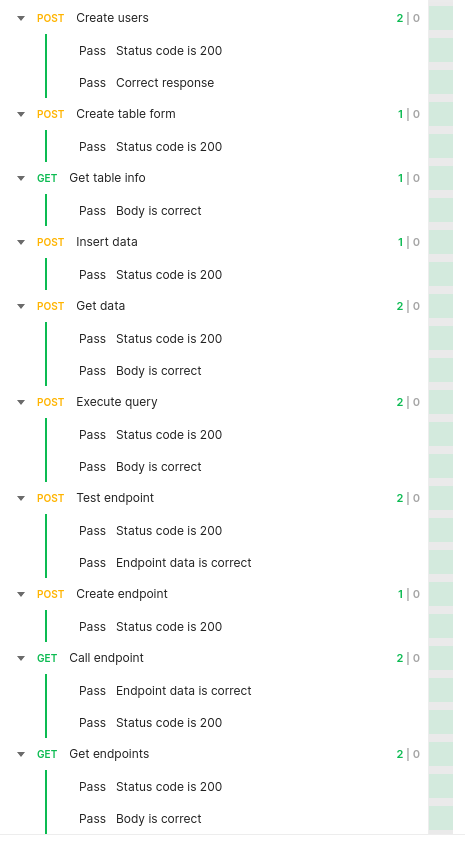
\includegraphics[width=0.6\textwidth]{./img/postman_test_exec.png}
    \caption{Wykonanie testów integracyjnych w programie Postman}
    \label{postmanTestExec}
\end{figure}

\FloatBarrier

Wykonanie testów integracyjnych powinno odbywać się po uruchomieniu aplikacji
backend po raz pierwszy z pustą bazą danych. Stan aplikacji zostaje zachowany
podczas całego działania testów integracyjnych. Działanie to można opisać
następująco:

\begin{enumerate}

    \item Create users - test wysyła do serwera polecenie stworzenia
        użytkowników, sprawdza czy odpowiedź jest poprawna.

    \item Create table form - test wysyła do serwera polecenie stworzenia
        tabeli. Polecenie nie zawiera zapytania SQL. Jest to wariant polecenia,
        który wysyła aplikacja frontend przy tworzeniu nowego typu danych za
        pomocą formularza.

    \item Get table info - test wysyła do serwera zapytanie o informacje o
        tabelach zawartych w bazie danych. Test sprawdza, czy odpowiedź zawiera
        dane o tabeli stworzonej w teście 2.

    \item Insert data - test wysyła do serwera polecenie dodania danych do
        tabeli. Jest to wariant polecenia, jakie wysyła aplikacja frontend przy
        dodawaniu danych za pomocą formularza.

    \item Get data - test wysyła do serwera zapytanie o informacje zawarte w
        tabeli stworzonej w teście 2. Jest to wariant zapytania, jakie wysyła
        aplikacja frontend w edytorze danych opartym o formularze. Test
        sprawdza, czy dane są takie same, jak te dodane do tabeli w teście 4.

    \item Execute query - test wysyła do serwera zapytanie HTTP z zapytaniami
        SQL. Test wysyła zapytanie tworzące nowe dane w tabeli stworzonej w
        teście 2 oraz zwracające stworzone dane. Zapytanie zostało umieszczone
        poniżej.

        \begin{verbatim}
insert into test_table_one (name, age)
    values ('Adam Nowak', 42)
    returning name, age::text
        \end{verbatim}

        Ponadto, zapytanie zawiera zapytanie SQL wykonywane przed i po wykonaniu
        drzewa zapytań. Jest to zapytanie pobierające wartości z kolumny
        \verb|name| z tabeli \verb|test_table_one|. Test sprawdza czy zapytanie
        zostało poprawnie wykonane oraz czy wartości zapytania wykonywanego
        przed i po drzewie zapytań są poprawne.

    \item Test endpoint - test wysyła do serwera zapytanie będące wariantem
        zapytania, jakie wysyła aplikacja frontend w celu przetestowania
        tworzonego punktu końcowego.

\end{enumerate}
